\documentclass{article}

\usepackage{graphicx}

\title{CS 6660: Scaling Projective Dynamics on GPU}
\author{Will Usher and Pavol Klacansky}

\begin{document}
\maketitle

\section{Introduction}
Projective Dynamics~\cite{Bouaziz14} solves continuum mechanics system using
local projective step and global implicit solver step. The local step projects
to constraints valid state and has no interdata dependencies, thus is data
parallel. The global step solves a system of linear equations which represent
the projections and external forces (including inertia). We choose to explore
parallelization of global step, as the local step is trivial, by implementing
a special case of projective dynamics, a mass-spring system~\cite{Liu13}


\section{Direct Solvers}
Direct solvers are difficult to parallelize due interdependencies and we
expected low performance. We used cuSPARSE to solve the global step and it
was significantly slower than conjugate gradient.


\section{Iterative Solvers}
The matrix $A$ is SPD, thus we used conjugate gradient from ViennaCL library
with various preconditioners. From our tests, after certian size (256x256)
the algebraic multigrid preconditioner outperforms Jacobi or none,
see Figure~.

The state-of-the art iterative solver seems to be~\cite{Wang15} and we tried
to implement it but we could not get it working. Another pitfal of this method
is many input parameters to set up and tweak.


\section{Domain Decomposition}
In previous sections we noted that direct solvers are mostly serial (PARDISO
was getting less than 2x speedup on 4 cores with 8 HW threads). Furthermore,
the block Jacobi with preconditioner direct solver for each block scaled
poorly, even with preconditioned blocks on the matrix diagonal. We postulate
the scaling is affected by limited memory bandwitdth and load imbalance, as
the columns in the individual rows are executed in serial.

We also tested some basic (incorrect) domain decompositions, one where two
pieces of cloth overlap and each acts as attachment constraint for the other.
This approach is data parallel as the attachments are updated after both
cloths were solved.

The other approach is to use third cloth to glue the two pieces and do a
fan-in (i.e. solve two pieces in parallel, then solve middle piece). We did
not set the vertex weights properly (how to do it?), thus our cloth exploded
as the middle step inserts energy by pulling too much.


\section{Conclusion}
During this project we have explored direct and iterative solvers on GPU,
simple domain decompositions, and parallel block Jacobi solver on CPU.
Figure~\ref{fig:amg_direct} compares the best performing solver on CPU and
GPU.
We found out, that iterative solvers do not perform well in PD, since as the
timestep gets larger, the iteration count increases sublinearly, thus the
direct solver will eventually outperform the iterative solver.

\begin{figure}[htb!]
        \centering
        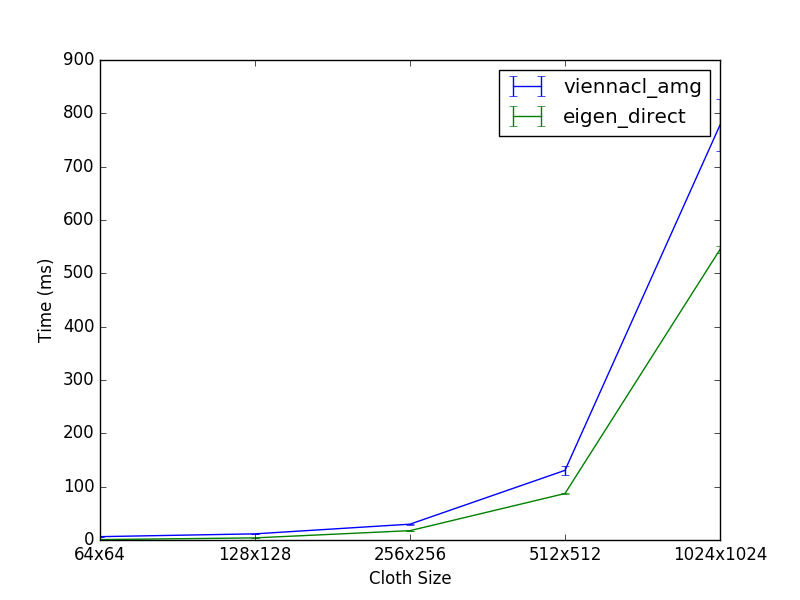
\includegraphics[width=\linewidth]{img/amg_direct.png}
        \caption{Direct solver on CPU compares to CG with AMG preconditioner
                 on GPU.}
        \label{fig:amg_direct}
\end{figure}


We conclude the best performing is Chebyshev approach by Wang~\cite{Wang15},
which outperforms both single core direct solver (1.5x) and AMG CG on GPU (3x).
Unfortunately, we tried and failed to get it working in our framework, thus
the comparison is based only on number of points ($L$ matrix). The major
downside of Chebyshev method is multitude of tweakable parameters which need
to be tuned for the application.


\bibliography{report}{}
\bibliographystyle{plain}

\end{document}
